%-*- mode: LaTex; outline-regexp: "\\\\section\\|\\\\subsection";fill-column: 80; -*-
\documentclass[12pt]{article}
\usepackage[longnamesfirst]{natbib}
\usepackage[usenames]{color}
\usepackage{graphicx}  % Macintosh pdf files for figures
\usepackage{amssymb}   % Real number symbol {\Bbb R}
\usepackage{bbm}
\input{../../standard}

% --- margins
\usepackage{../sty/simplemargins}
\setleftmargin{1in}   % 1 inch is NSF legal minimum
\setrightmargin{1in}  % 1 inch is NSF legal minimum
\settopmargin{1in}    % 1 inch is NSF legal minimum
\setbottommargin{1in} % 1 inch is NSF legal minimum

% --- Paragraph split, indents
\setlength{\parskip}{0.20in}
\setlength{\parindent}{0.20in}

% --- Line spacing
\renewcommand{\baselinestretch}{1.5}

% --- page numbers
\pagestyle{empty}  % so no page numbers

% --- Hypthenation
\sloppy  % fewer hyphenated
\hyphenation{stan-dard}
\hyphenation{among}

% --- Customized commands, abbreviations
\newcommand{\TIT}{{\it  {\tiny Leverage (\today)}}}

% --- Header
\pagestyle{myheadings}
\markright{\TIT}

% --- Title

\title{ Leveraged Collinearity and Model Selection }
\date{\today}

%%%%%%%%%%%%%%%%%%%%%%%%%%%%%%%%%%%%%%%

\begin{document}
% \maketitle 


%--------------------------------------------------------------------------
\section{ To Do }
%--------------------------------------------------------------------------

\begin{itemize}

 \item Link back to earlier work in which CVSS and AIC were pointing to
 different models. The results here might be a good explanation of that
 phenomenon.

 \item Figure out what it means to have 'comparable' situations among IID,
 leveraged cases, and autoregressive models.

 \item Decide how to handle the intercept. It mucks up the comparison analysis
 later since $\ev X'X$ has that non-stochastic leading $n$.

\end{itemize}


%--------------------------------------------------------------------------
\section{ Motivation }
\label{sec:motivation}
%--------------------------------------------------------------------------

 This problem is motivated by selecting features for a regression in text
 analysis.  The features for this regression are derived from the singular value
 decomposition of the document/term matrix of a large collection of text
 documents.  The value of the response is a characteristic of the subject of the
 document.  In our application, documents are real-estate listings that verbally
 describe properties.  The response is the listed price of the home.  The
 regression features are eigenwords from the text of a collection of listings,
 singular vectors from the document/term matrix.  Rather than try to find the
 best subset, the monotone predictive value of these features suggests picking
 them in order, much like one does with an autoregression (albeit on a larger
 scale).  Should we use the first 10, 30, or 50 singular vectors (eigenwords) as
 features?  The problem is complicated by the presence of outliers produced by
 the decomposition.  Given the Ziphian distribution associated with text,
 outliers are to be expected.


 More generally, leveraged observations produce surprising effects on regression
 models, particularly by producing a form of collinearity among the explanatory
 features.  Leveraged observations in our setting are simply rows of the design
 matrix $X$ that have large variance compared to typical rows.


%--------------------------------------------------------------------------
\section{ Stylized Problem }
\label{sec:problem}
%--------------------------------------------------------------------------

 The following example illustrates what can happen.  Let $(X_{i1}, \ldots,
 X_{ip})'$ for $i = 1,\ldots,n$ denote a vector of $p$ independent Gaussian
 variables.  These vectors form the rows of the design matrix $X$ in a linear
 regression.  To produce the leverage effects observed in text regressions, we
 assume the first $n_o$ observations have variance $\sigma_o^2$, and the
 remaining observations have variance 1:
 \begin{equation}
    X_{ij} \sim \left\{ \begin{array}{cc}
              N(0,\sigma_o^2), & i \le n_o \cr
              N(0,1)    , & n_o < i \le n \;.
   \end{array} \right.
 \label{eq:Xij}
 \end{equation}
 The observations are independent, but not identically distributed.  The model
 for the response is the usual Gaussian regression with {\em constant} error
 variance.  If we let $X_j$ with a single subscript denote the $j$th column of
the $n \times p$ matrix $X$ with elements$X_{ij}$, then the regression model is
 \begin{equation}
   Y = \beta_0 + \beta_1 X_{1} + \cdots + \beta_p X_{p} + \sigma \ep,
        \quad \ep_i \sim N(0,1) \;.   
 \label{eq:Yi}
 \end{equation}
 Notice that the model is {\em not} heteroscedastic; rather, the changing
 variances occur among the rows of $X$.


 Now suppose that we know that only the first $k$ elements of $\beta$ are
 non-zero.  How should we pick the best fitting regression, one that minimizes
 the squared error of prediction?  As will become clear, this question is not
 well-posed.  A popular choice for this context is pick for $k$ the model that
 minimizes \aic, which we illustrate with a simulated example.  For this
 example, we observe $n = 2000$ cases of $p = 150$ available features, with
 $n_o=50$ leverage points with standard deviation $\sigma_o = 100$.  Before
 continuing to the response, we note that the presence of these leverage points
 produces a surprising amount of collinearity given that the design points are
 independent.  Figure \ref{fig:cn} graphs the condition number of the leading
 columns of $X$, varying the number of columns included.  (The condition number
 is the ratio of the largest to smallest singular value of a non-square matrix.)
  The left frame shows the condition number if $\sigma_o = 1$ (\ie, without
 leverage points); the condition number grows roughly linearly in the number of
 columns (slope $\approx 0.0046$).  The right frame of Figure \ref{fig:cn} shows
 the condition number in the context of our simulated data with $n_o = 50$ and
 $\sigma_o = 100$.  Again, the condition number increases linearly, but with a
 much steeper slope near 0.26.  But for the scale of the y-axis, the figures are
 almost identical.  The linear growth in the condition number persists for
 matrices with more than $n_o$ columns; larger matrices do not quickly
 ``outgrow'' the influence of the leverage points.  The amount of collinearity
 grows at a steady fixed rate (for these dimensions) as the number of columns
 increases.

 \begin{figure}
 \caption{ Condition numbers for matrices with increasing numbers of columns,
 with with no leveraged outliers (left) or with $n_o=50$ leveraged outliers with
 standard deviation $\sigma_o=100$ (right). } 
 \label{fig:cn}
 \centerline{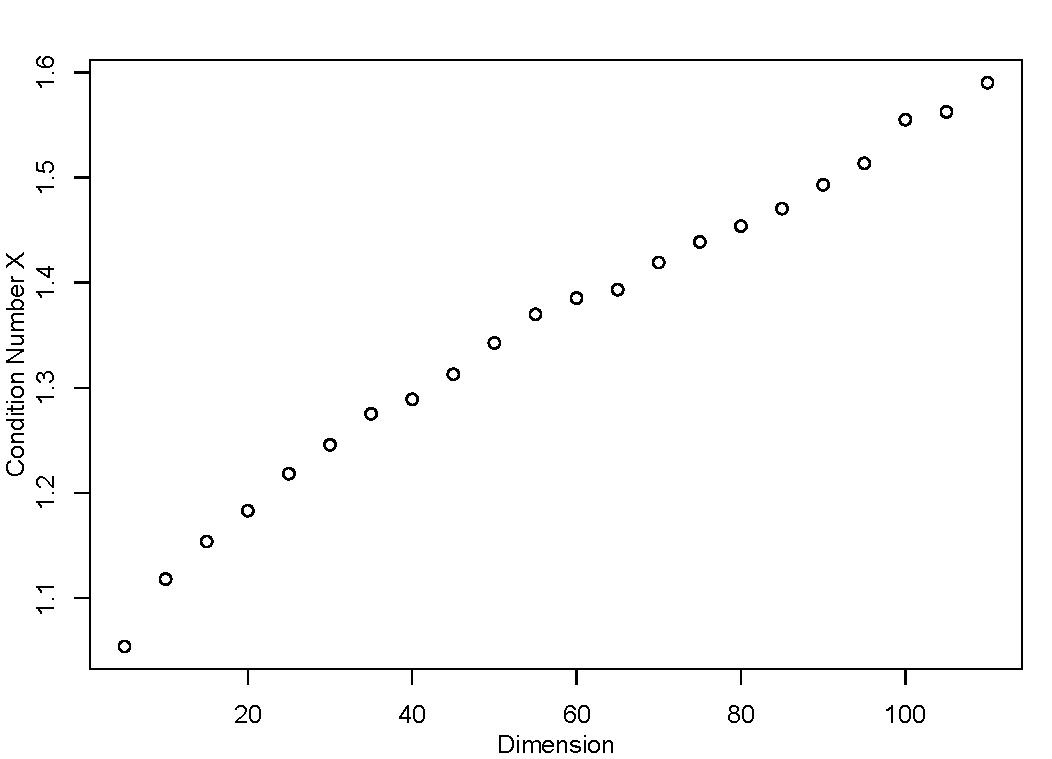
\includegraphics[width=2.5in]{figures/cn1.pdf}
             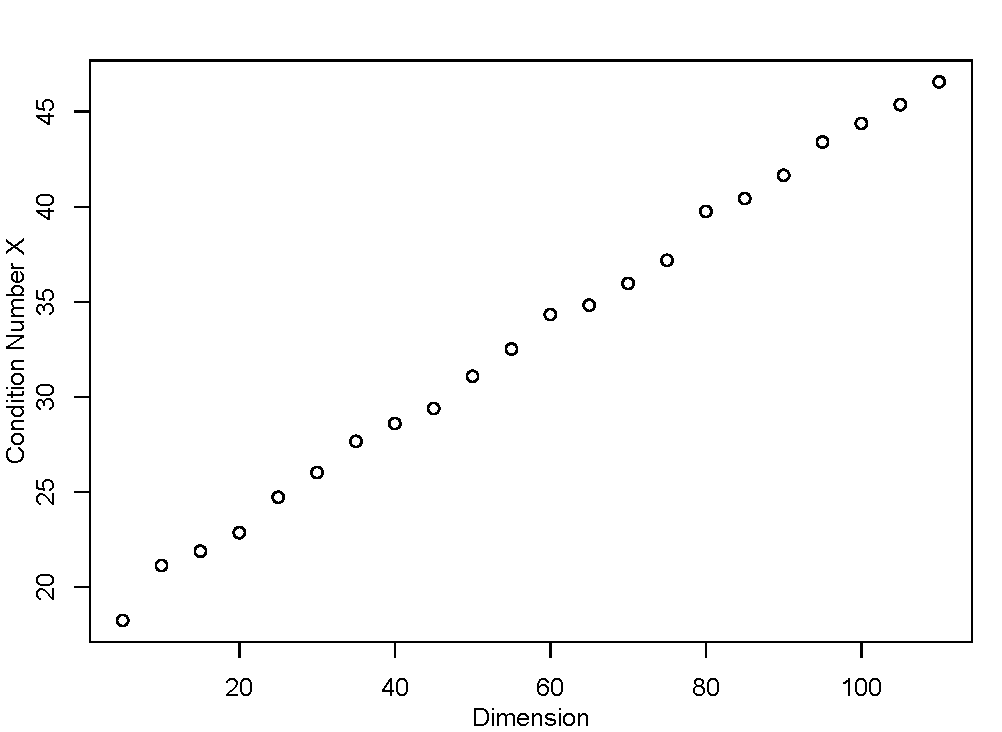
\includegraphics[width=2.5in]{figures/cn100.pdf}}
 \end{figure}


 Figure \ref{fig:example1} shows the impact of these leverage points on the
 problem of picking a model.  For this illustration, $k = 75$ features are
 predictive (\ie, have non-zero regression coefficient).  We set the error
 variance to $\sigma=1$ and $\beta_j = c$ for $j = 1,\ldots,k$, with $c$ chosen
 so that these coefficients lie, on average, about 5 standard errors from 0 when
 fitting the model with all 75 features included.  As such, these features are
 very significant effects, and $R^2 \approx 0.53$ for the fully specified model
 that uses $X_1,\ldots,X_{75}$.  The top frame of Figure \ref{fig:example1}
 plots two versions of \aic\ for models of increasing size.  The White version
 of \aic\ uses a heteroscedastic consistent estimate of the variance of
 $\hat\beta$ rather than the usual expression. (We also use the estimate of
 $\sigma^2$ from the prior model with $j-1$ features when computing \aic\ for
 the model with $j$ features.)  Because these do not lie in the same range, we
 rescaled both \aic\ statistics to lie on a common range for visual comparisons.
  The version of \aic\ corrected for heteroscedasticity shows a dramatic valley
 and relatively steep increase past its minimum.  Though showing different
 trends, the two versions of \aic\ pick a model with about 50 features,
 substantially fewer than $k=75$ and instead matching the number of leverage
 points.  The vertical gray line in this and other figures highlights the number
 of leveraged outliers in the data (in this case, $n_o=50$).  Other colored
 vertical segments denote the position of the minimum value of each series,
 identifying the ``best'' model as judged by each metric.

 \begin{figure}
 \caption{ Simulation of \aic\ (normal in blue and heteroscedastic consistent,
 top) and model loss and mean squared prediction errors (bottom), in the
 presence of leverage points.  The loss is shown in black, with the fixed-design
 mean squared error (blue, equation \ref{eq:fixed}) and the corresponding
 random-design error (magenta, equation \ref{eq:random}). }
 \label{fig:example1}
  \centerline{ 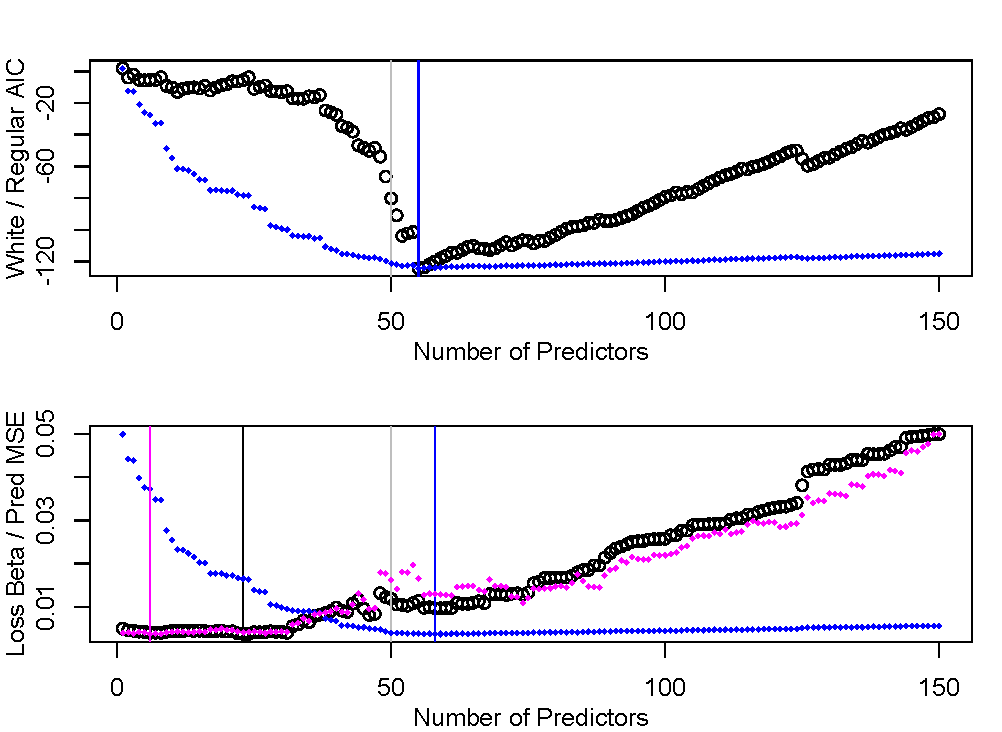
\includegraphics[width=5in]{figures/example1.pdf} }
 \end{figure}

 The lower panel of Figure \ref{fig:example1} shows how well each model in this
 sequence of fits performs.  Whereas both versions of \aic\ are computable; the
 lower panel graphs unobservable random variables that are computable only
 because we simulated these data from known models.  The black points in the
 figure show the loss when estimating $\beta$.  Let $X_{0:j}$ refer to a matrix
 comprised of a column of 1's followed by the first $j$ columns of $X$, and
 similarly let $\beta_{0:j}$ and $\hat\beta_{0:j}$ denote the corresponding true
 coefficients and least squares estimates (including the intercept).  The model
 loss (black points) is then the sequence
 \begin{equation}
    \normsq{ \beta_{0:j} - \hat\beta_{0:j}} \;, \quad j = 1,\ldots,150 \;.
 \label{eq:loss}
 \end{equation}
 The sequence of blue points in the figure are the mean squared errors under a
 fixed-$X$ design, computed as
 \begin{equation}
    \mbox{Fixed-Design MSE:  } \normsq{ X_{0:j}(\hat\beta_{0:j}-\beta_{0:j}) }   
 \label{eq:fixed}
 \end{equation} 
 Again, for the sake of comparison, the lower panel of Figure \ref{fig:example1}
 graphs the series using a common y-axis.  The fixed-design MSE presumes that
 were we to predict new data, the new observations would have the same values of
 the observed model features.  The sequence of fixed-design MSEs is highly
 correlated with the trend of the usual \aic\ statistic shown in the upper panel
 of Figure \ref{fig:example1}.  In contrast, the random-design mean squared
 error shown in magenta in Figure \ref{fig:example1} measures the accuracy in
 the more realistic context in which we predict new data from the same
 population, but not at the same values of the explanatory variables.  This MSE
 is computed by independently simulating a second realization of the design
 matrix from the same process, including the same choices for simulating
 leverage points, and computing the prediction error obtained at these values of
 the model features.  If we denote an independent realization of $X$ by
 $\widetilde{X}$, then the magenta points in the lower panel of Figure
 \ref{fig:example1} show
 \begin{equation}
    \mbox{Random Design MSE:  } 
    \normsq{ \widetilde{X}_{0:j}(\hat\beta_{0:j}-\beta_{0:j}) }   
 \label{eq:random}
 \end{equation} 
 The random design MSE closely mimics the trend in the loss, which is
 proportional to its expectation (over the distribution of $X$):
 \begin{eqnarray}
  \ev \normsq{\widetilde{X}_{0:j}(\hat\beta_{0:j} - \beta_{0:j})}
   &=& \ev (\hat\beta_{0:j} - \beta_{0:j})' \widetilde{X}_{0:j}' 
            \widetilde{X}_{0:j} (\hat\beta_{0:j} - \beta_{0:j}) \cr
   &=& \ev \tr \widetilde{X}_{0:j}'\widetilde{X}_{0:j} 
           (\hat\beta_{0:j} - \beta_{0:j}) (\hat\beta_{0:j} - \beta_{0:j})' \cr
   &=& \tr \ev \widetilde{X}_{0:j}'\widetilde{X}_{0:j} 
           (\hat\beta_{0:j} - \beta_{0:j}) (\hat\beta_{0:j} - \beta_{0:j})' \cr
   &=& \tr \ev (\widetilde{X}_{0:j}'\widetilde{X}_{0:j})
           \ev ((\hat\beta_{0:j} - \beta_{0:j})(\hat\beta_{0:j} - \beta_{0:j})') \cr
   &=& \tr D_j(n,c) 
           \ev ((\hat\beta_{0:j} - \beta_{0:j})(\hat\beta_{0:j} - \beta_{0:j})') \cr
   &\approx& c \; 
           \ev (\hat\beta_{0:j} - \beta_{0:j})'(\hat\beta_{0:j} - \beta_{0:j})\;,
 \end{eqnarray}
 where $D_j(n,c)$ is a diagonal matrix with leading diagonal element $n$
 followed by $j$ copies of the constant $c = n_o \sigma_o^2 + (n - n_o)$.  The
 approximation results from replacing $n$ by $c$ in this leading diagonal
 matrix.

 
 In the presence of leverage points, \aic\ thus picks the model that predicts
 well at the {\em observed} design points.  After all, that's the only data
 visible.  What we more often experience in practice, however, is the behavior
 of the random-design MSE.  Out-of-sample leverage points possess a very
 different configuration than those observed in-sample, and the model cannot
 predict this new configuration so well as that which was observed.  In this
 sense, \aic\ answers one question (evidently pretty well), but it may not be
 the question we need to answer.


 These problems vanish without the leverage points, even in models with
 collinearity among the features.  Figure \ref{fig:example2} shows the same
 statistics and random variables as Figure \ref{fig:example1}, but for data that
 lack the high leverage points. Again, $b=2000$ with $p=150$ possible features,
 of which the first 75 have non-zero coefficients.  Both versions of \aic\ align
 closely and pick the correct model with $75$ features, and all of the error
 measures in the second panel agree.

 \begin{figure}
 \caption{ Simulation of \aic\ (normal in blue and heteroscedastic consistent,
 top) and model loss and mean squared prediction errors (bottom), without
leverage points. }
 \label{fig:example2}
  \centerline{ 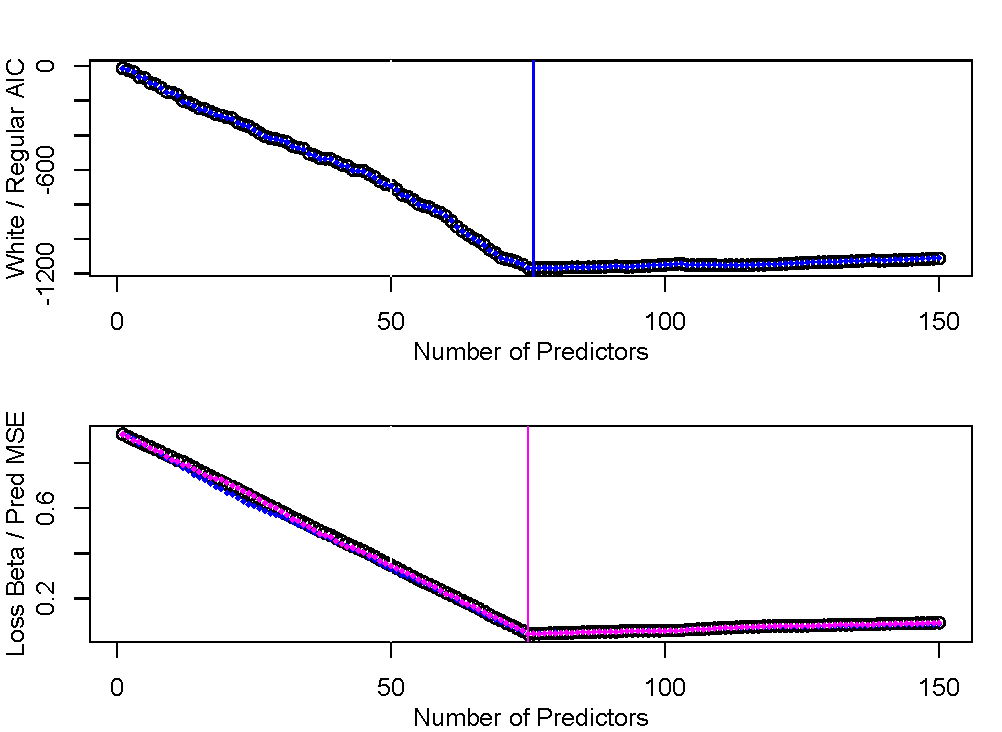
\includegraphics[width=5in]{figures/example2.pdf} }
 \end{figure}


 \ras{The following results are dodgy: depends a lot on how you make the data. }

 An obvious question to pose at this point is to ask: How do these plots look
 under other forms of collinearity?  For example, a common model used to
 generate correlated predictors is the first-order autoregression, in which
 $\Corr(X_j,X_k) = \phi^{|j-k|}$ for $|\phi| < 1$.  Figure \ref{fig:example3}
 shows the two versions of \aic\ and mean squared errors as in Figures
 \ref{fig:example1} and \ref{fig:example2}, but with autoregressive dependence
 among the columns of $X$.  Specifically, we set $\phi=0.935$ so that the
 condition number of $X$ approximates that produced by the leveraged outliers in
 the first example.  In this setting, the two versions of \aic\ closely agree,
 and both pick the correct model with $k = 75$ features.  The fixed- and
 random-design mean squared errors are also very similar with minimum values
 near $k=75$.  The difference lies in the trend produced by the squared loss in
 estimating $\beta$.  While the minimum loss occurs for a model near those that
 minimize the two forms of the MSE, the trend in the loss is rather different
 and more volatile.

 \begin{figure}
 \caption{ Simulation of \aic\ (normal in blue and heteroscedastic consistent,
 top) and model loss and mean squared prediction errors (bottom), when fitting a
 model with autoregressive dependence among the explanatory features. }
 \label{fig:example3}
  \centerline{ 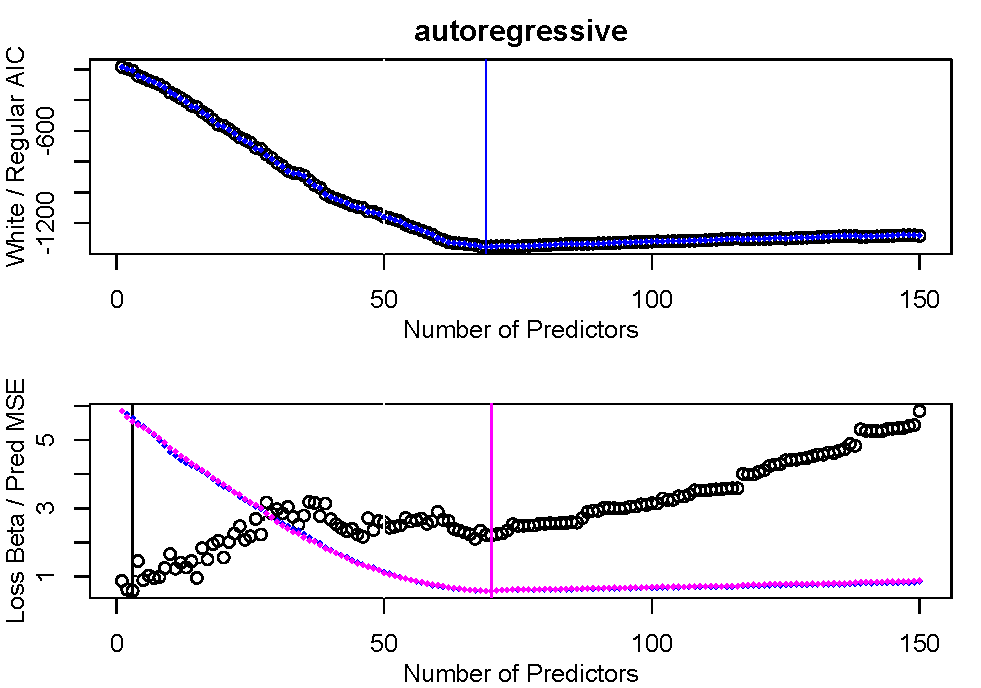
\includegraphics[width=5in]{figures/example3.pdf} }
 \end{figure}



%--------------------------------------------------------------------------
\section{ xx }
\label{sec:}
%--------------------------------------------------------------------------


%--------------------------------------------------------------------------
\section{ xx }
\label{sec:}
%--------------------------------------------------------------------------



%--------------------------------------------------------------------------
\section{ Derivations  }
\label{sec:derive}
%--------------------------------------------------------------------------


%--------------------------------------------------------------------------
% References
%--------------------------------------------------------------------------

\bibliography{../../../references/stat,../../../references/TextPapers/text}
\bibliographystyle{../bst/ims}

\end{document} %==========================================================
